\state{}{
	A long-wavelength optical phonon in an insulating ionic solid is described by the following equation of motion:
	\eqn{ODE}{
		M \vudd + K \vuu = Q \vE,
	}
	where $\vuu$ is the atomic displacement, $M$ the mass, $K$ a local restoring force, and $\vE$ is the electric field.  A displacement of the ions by $\vuu$ results in a polarization
	\eqn{P}{
		\vP = n Q \vuu,
	}
	where $n$ is the density of the ions, and $Q$ their effective charge.  We will consider only longitudinal modes, where $\vD$, $\vE$, $\vuu$ are all parallel.
}

\prob{ \label{3a}
	Neglecting any further electronic response of the solid, calculate the response of the phonon mode to a uniform external electric displacement field $\vD = \epso \vE + \vP$, oscillating with a frequency $\omg$.  Hence show that the phonon contribution to the frequency-dependent dielectric function, defined by $D = \epsion \epso E$ may be written
	\eqn{show3a}{
		\epsionomg = 1 - \frac{\OmgP^2}{\omg^2 - \Omgo^2},
	}
	giving formulae for $\OmgP$ and $\Omgo$ in terms of the constants $M$, $K$, $n$, and $Q$.
}

\sol{
	Substituting $\vE = (\vD - \vP) / \epso$ and Eq.~\refeq{P} into Eq.~\refeq{ODE}, we have~[lecture notes, p.~75]
	\eqn{ODE2}{
		M \vudd + K \vuu = \frac{Q}{\epso} \vD - \frac{n Q}{\epso} \vuu
		\qimplies
		\epso M \vudd + \paren{ \epso K + n Q } \vuu = Q \vD.
	}
	The susceptibility or response function $\chiomg$ is given by~\cite[p.~185]{Griffiths}
	\eqn{response}{
		\vP = \epso \chi \vE.
	}
	We recall that differentiating in the time domain is equivalent to multiplying by $i \omg$ in the frequency domain~\cite{Fourier}:
	\eq{
		\cF_x [ f^{(n)}(x) ](\omg) = (i \omg)^n \cF [ f(x) ](\omg).
	}
	Then we can easily Fourier transform both sides of Eq.~\refeq{ODE}.  Let $x \equiv \epso K + n Q$.  Then
	\eq{
		Q \Domg = \epso M (i \omg)^2 \uomg + x \uomg
		= \paren{ x - \omg^2 \epso M } \uomg
		\qimplies
		\uomg = \frac{Q \Domg}{x - \epso M \omg^2}.
	}
	Feeding this into Eq.~\refeq{P}, we have
	\eq{
		\vP = \frac{n Q^2 \Domg}{x - \epso M \omg^2}
	}
	By Eq.~\refeq{response} and $D = \epsion \epso E$, then, the response function is
	\eq{
		\ans{ \chiomg = \frac{n Q^2}{\epso K + n Q - \epso M \omg^2}. }
	}
	The dielectric function is defined by $\eps \equiv 1 + \chi$~\cite[p.~186]{Griffiths}.  So the phonon contribution to the dielectric function is
	\eq{
		\epsionomg = 1 + \frac{n Q^2}{\epso K + n Q - \epso M \omg^2}
		= 1 - \frac{n Q^2}{\epso M \omg^2 - (\epso K + n Q)}
		= 1 - \frac{n Q^2 / \epso M}{\omg^2 - (\epso K + n Q) / \epso M},
	}
	or
	\eq{
		\ans{ \epsionomg = 1 - \frac{\OmgP^2}{\omg^2 - \Omgo^2} }
	}
	where
	\ans{\al{
		\OmgP &= \sqrt{\frac{n Q^2}{\epso M}}, &
		\Omgo &= \sqrt{\frac{\epso K + n Q}{\epso M}}
	}}%
	as we wanted to show. \qed
}



\prob{
	Figure~\ref{f3} shows measurements of the frequency squared of an optical phonon in an insulating oxide (solid line) and measurements of the reciprocal of the static dielectric constant $1 / \eps = 1 / \epsionomgo$ (dotted-dashed line) in the same material.  Using the model above, estimate the ion plasma frequency $\OmgP$ and discuss whether the magnitude of your result seems appropriate for a typical ionic solid.
	
	\begin{figure}[b!] \centering
		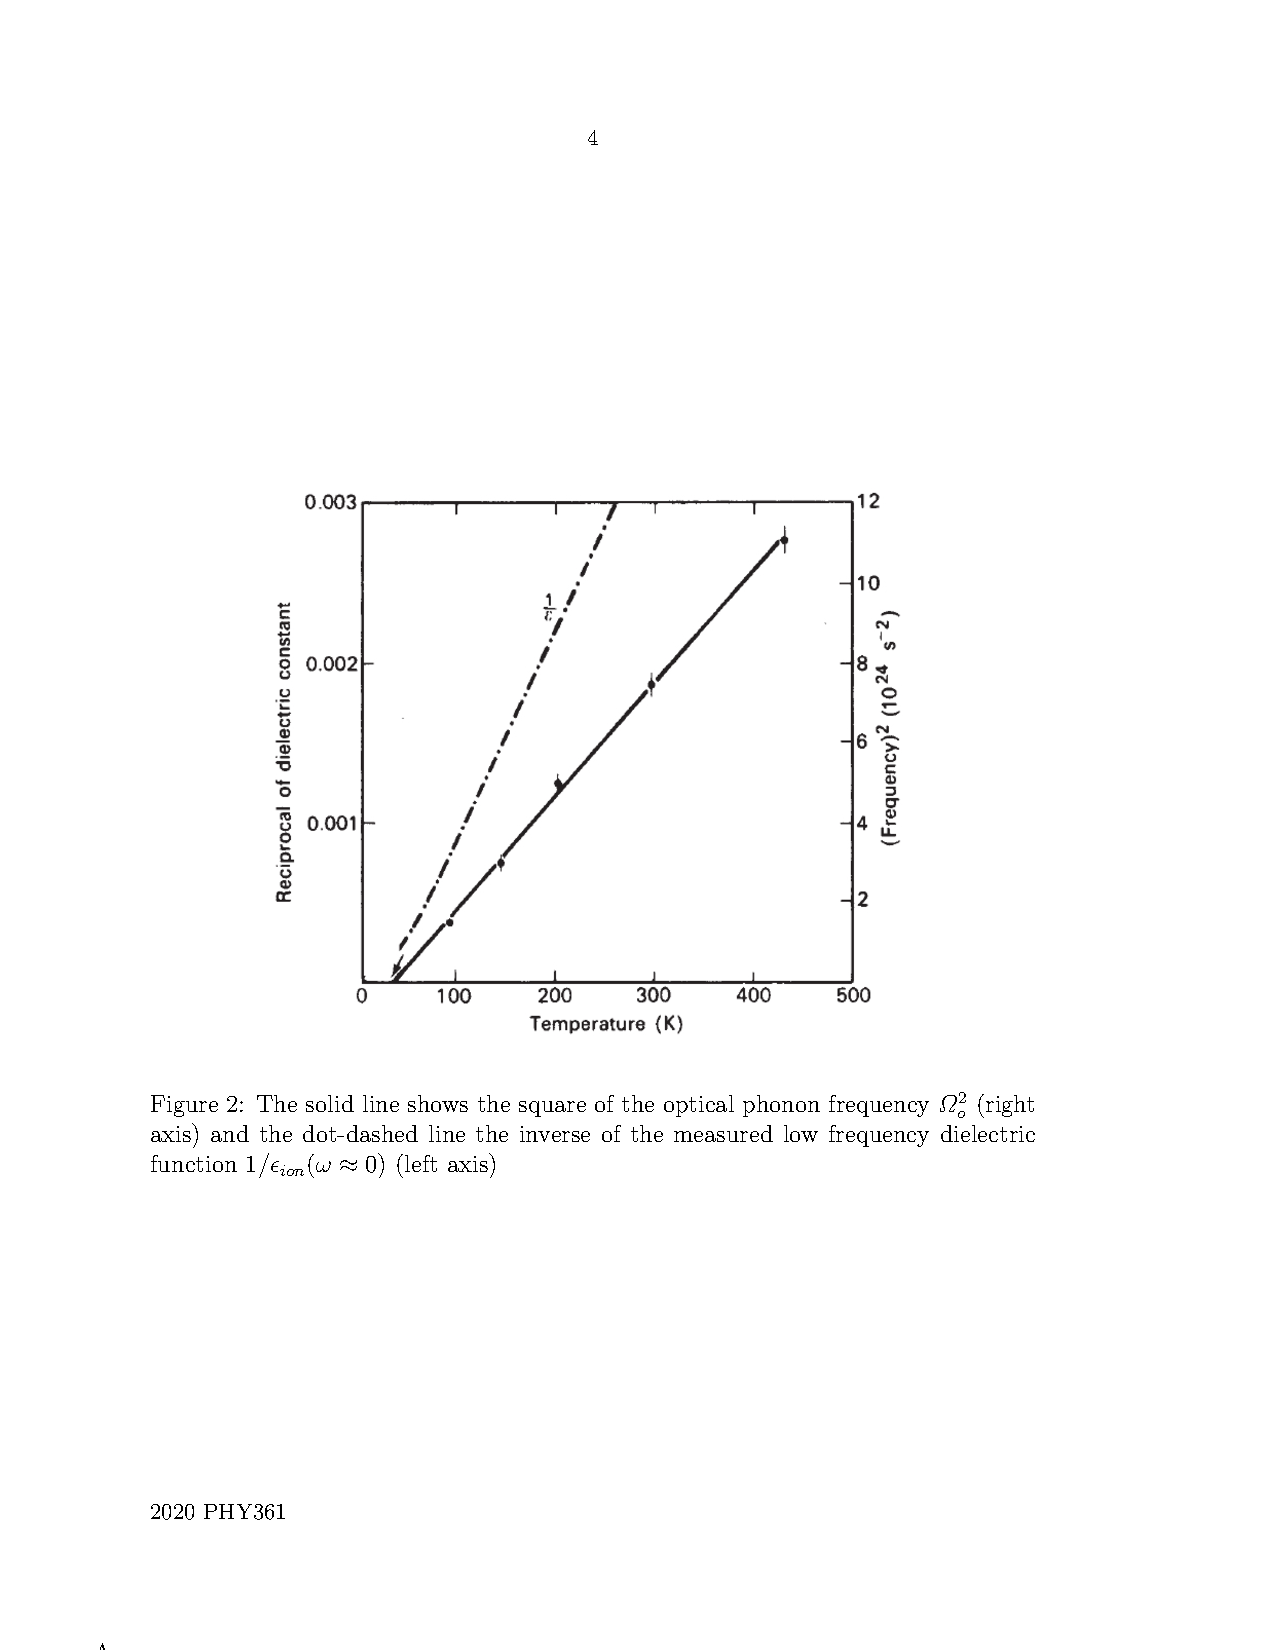
\includegraphics[width=0.5\textwidth,trim=4.5cm 10cm 6cm 8cm,clip]{fig2}
		\caption{The solid line shows the square of the optical phonon frequency $\Omgo^2$~(right axis) and the dot-dashed line the inverse of the measured low frequency dielectric function $1 / \epsionomgo$~(left axis).}
		\label{f3}
	\end{figure}
}

\sol{
	From Eq.~\refeq{show3a},
	\eq{
		\epsionomgo = 1 + \frac{\OmgP^2}{\Omgo^2}
		\qimplies
		\OmgP = \sqrt{\Omgo^2 (\epsionomgo - 1)}.
	}
	Inspecting Fig.~\ref{f3}, it appears that $\Omgo^2 \approx \OmgoSI$ when $1 / \eps \approx 0.002$ (or $\eps \approx 500$) slightly below \SI{200}{\kelvin}.  Plugging in these values,
	\eq{
		\OmgP \approx \sqrt{ (\OmgoSI) (500 - 1) }
		\approx 500 \sqrt{\OmgoSI}
		\approx \ans{ \OmgPSI. }
	}
	This is above the visible frequency range.  Assuming it can be said in general that a material reflects light of all frequencies below the plasma frequency (as we discovered for the Drude model in question~5.3 of the homework), then our material would be highly reflective at optical frequencies.  This is expected for a metal, but not for an insulator like the ionic solid in the problem.  So the magnitude of this result does not seem quite appropriate, though it is not too far off.  We would expect it to be at least one order of magnitude smaller in order not to reflect visible light.  
}



\prob{
	Explain how the extrapolated vanishing of the optical phonon frequency at low temperatures, marked by the arrow in the figure, is indicative of a phase transition.
}

\sol{
	As $\Omgo$ decreases with temperature, the crystal lattice is changing as well, since the phonon frequencies depend on how the nearby ions are arranged.  Say the lattice has a particular structure (here, cubic) with a particular phonon dispersion at $T \approx \SI{400}{\kelvin}$, and a different structure (not cubic) below $\Tc$, the temperature at which the optical phonon frequency vanishes.  The low-temperature structure may have a completely different phonon dispersion than the high-temperature structure.  As the temperature decreases and the crystal morphs from the high-temperature to the low-temperature structure, the occupation of the high-temperature phonon states will decrease in favor of the low-temperature phonon states.  When the temperature reaches $\Tc$ and the crystal has fully transformed into the low-temperature structure, the optical phonon frequency of the high-temperature structure completely disappears.  This is a structural phase transition~\cite[p.~467]{Kittel}.
}



\prob{
	Construct a phenomenological Landau theory for the free energy of the solid as a power series expansion in the polarization, consistent with cubic symmetry.
}

\sol{
	Since we are constructing a Landau theory with polarization as the order parameter, it is likely our ionic solid is ferroelectric, which is consistent with the structural phase transition~\cite[pp.~469--470]{Kittel}.  Since $\Omgo = 0$ at $\Tc$, $\chiomgo = \OmgP^2 / \Omgo^2$ diverges at the critical temperature.  This is characteristic of a second-order phase transition~[lecture notes, p.~79].
	
	We can write the free energy in the form
	\eq{
		\cF = \frac{a}{2} P^2 + \frac{b}{4} P^4 + \frac{c}{6} P^6 + \cdots,
	}
	where $P$, representing the polarization, can be written as a scalar instead of a three-dimensional vector since it may only point in a symmetry direction of the lattice~[lecture notes, p.~103].  The coefficient $a = \ao (T - \Tc)$ where $\ao > 0$ is a constant~\cite{Landau}.   For a second-order transition, $b > 0$, and since the $\order{P^4}$ term contributes much more than the $\order{P^6}$ term, so we may neglect it~\cite[p.~475]{Kittel}.  Our theory is then
	\eq{
		\ans{ \cF = \frac{a}{2} P^2 + \frac{b}{4} P^4 + \cdots, }
	}
	where
	\ans{\al{
		a &= \ao (T - \Tc), &
		\ao &> 0, &
		b &> 0.
	}}%
	\vfix
}



\prob{
	Use your model to predict how the phonon frequency $\Omgo$ and static dielectric constant $\epsion$ would vary with temperature below the critical temperature.
}

\sol{
	The equilibrium $\PT$ occurs at the minima of $\cF$, where $\dv*{\cF}{P} = 0$~\cite[p.~475]{Kittel}:
	\eq{
		\dv{\cF}{P} = a P + b P^3 = 0.
	}
	This implies
	\al{
		P &= 0, &
		P &= \pm \sqrt{-\frac{a}{b}}.
	}
	Note, however, that $P = 0$ is a local maximum of $\cF$ if $T < \Tc$:
	\eq{
		\left. \dv[2]{\cF}{P} \right|_{P = 0} = \brac{ a + 2 b P^2 }_{P = 0}
		= \ao (T - \Tc)
		< 0 \quad \text{when } T < \Tc.
	}
	However, the nonzero solution is imaginary for $T > \Tc$.  Thus the equilibrium $\PT$ is given by
	\aln{ \label{PT}
		\PT &= \pm \sqrt{\dfrac{\ao}{b} (\Tc - T)} &
		\text{when} \quad T &< \Tc.
	}
	By including in $\cF$ the energy of the polarization coupled to an external electric field $E$, we can determine the dielectric susceptibility $\chi = \dv*{P}{E}$ below the critical temperature~[lecture notes, p.~103].  With the addition of the coupling term~\cite[p.~475]{Kittel}:
	\eq{
		\cF = \frac{a}{2} P^2 + \frac{b}{4} P^4 - E P.
	}
	Then
	\eq{
		\dv{\cF}{P} = a P + b P^3 - E
		= 0.
	}
	Differentiating both sides by E, we find
	\eq{
		0 = a \dv{P}{E} + b \dv{P^3}{E} - 1
		= a \dv{P}{E} + b \dv{P^3}{P} \dv{P}{E} - 1
		= a \chi + 3 b P^2 \chi - 1,
	}
	which implies
	\aln{ \label{chiT}
		\chiT &= \frac{1}{a + 3 b P^2}
		= \frac{1}{\ao (T - \Tc) + 3 \ao (\Tc - T)}
		= \frac{1}{2 \ao (\Tc - T)} &
		\text{when} \quad T &< \Tc,
	}
	where we have used $\PT$ as defined in Eq.~\refeq{PT} and ignored the imaginary $\PT$.  Although this $\PT$ is evaluated at $E = 0$, we assume the difference is negligible from $\PT$ evaluated at small $E$~[lecture notes, p.~79].
	
	We know from \ref{3a} that $\eps \equiv 1 + \chi$ and $\chiomgo = \OmgP^2 / \Omgo^2$.  Then applying Eq.~\refeq{chiT} tells us
	\ans{\al{
		\Omgo(T) &= \frac{\OmgP}{\sqrt{\chiT}}
		= \OmgP \sqrt{2 \ao (\Tc - T)} &
		\text{when} \quad T &< \Tc
	}}%
	and
	\ans{\al{
		\epsion(T) &= 1 + \chiT
		= 1 + \frac{1}{2 \ao (\Tc - T)}&
		\text{when} \quad T &< \Tc.
	}}%
	\vfix
}